\documentclass[letterpaper]{article}
\usepackage[submission]{aaai2027}
\usepackage[hyphens]{url}
\usepackage{graphicx}
\urlstyle{rm}
\def\UrlFont{\rm}
\usepackage{natbib}
\usepackage{caption}
\frenchspacing

\usepackage{amsmath}
\usepackage{amssymb}
\usepackage{booktabs}
\usepackage{array}

\pdfinfo{/TemplateVersion (2027.1)}
\setcounter{secnumdepth}{0}

\title{When Short Trajectories Lie:\\Information-Induced Gradient Contraction in Multi-Agent RL}
\author{Anonymous Submission}
\affiliations{}

\begin{document}
\maketitle

\begin{abstract}
Short learning trajectories are routinely taken as evidence of stable convergence in reinforcement learning.
We show that, under partially observable multi-agent settings, they may instead signal a failure to learn.
When relational variables---teammate identity, role, or task assignment---are hidden, policy gradients that are individually informative across distinct relational contexts are projected onto a coarser observation space and may cancel.
%
We formalize this phenomenon as \textbf{Information-Induced Gradient Contraction (IIGC)}, derive a Pythagorean decomposition of relation-conditioned gradient energy, and introduce the \textbf{Relational Gradient Retention Ratio}, $\kappa$, which quantifies how much usable learning signal survives partial observability.
Combined with a drift-diffusion trajectory analysis, $\kappa$ yields a \textbf{Stable-or-Stuck diagnostic} that distinguishes genuine convergence from information-induced stagnation across four distinct training regimes.

We validate this framework across three multi-agent environments.
In 510K, a four-player card game with configurable cooperation structures, 22 PPO runs reveal that the hidden-relation regime produces the shortest behavioral trajectories ($0.293 \pm 0.049$), while revealing the same relations yields longer paths ($0.328 \pm 0.062$).
A visible-team ablation ($n=8$) isolates known-team information as the causal driver.
In a synthetic toy problem, $\kappa \approx 0$ with a wandering learning path and chance-level return---the path integral and $\kappa$ give opposite diagnoses.
In Overcooked with hidden partner roles, $\kappa$ correctly identifies gradient death ($\kappa = 0.000$) across all eight seeds.
Cross-algorithm $\kappa$ measurements distinguish policy-gradient, value-based, and actor-critic methods, revealing that policy-gradient methods are uniquely vulnerable to IIGC.
We contribute the IIGC framework, the $\kappa$ metric, and the Stable-or-Stuck diagnostic for MARL practitioners.
\end{abstract}


\section{Introduction}

Consider three multi-agent reinforcement learning (MARL) scenarios:

\begin{enumerate}
\item In a four-player card game, an agent wins by cooperating with a teammate whose identity is hidden---determined by a private card each player holds.
\item A chef in a crowded kitchen receives a different cooking partner each shift. The partner's role (cook vs.\ deliver) is hidden, requiring the chef to adapt on the fly.
\item An agent chooses between two actions. Reward arrives only when its action matches a hidden partner's type---but the agent never observes the partner.
\end{enumerate}

In each case, the agent faces \textbf{hidden relational information}: it cannot observe a critical variable (teammate identity, partner role, partner type) that determines the optimal policy.
How does this affect the training trajectory?

The conventional answer: hidden information complicates training, producing noisier, longer, more tortuous paths.
Our experiments on \textbf{510K}, a four-player Chinese trick-taking card game, initially confirmed this intuition---but in the \textit{opposite direction}.
%
Across 22 PPO runs spanning four rule variants, computing the \textbf{path integral}---the cumulative L2 distance traversed through a seven-dimensional behavioral feature space---revealed:
\textbf{stronger cooperation constraints produce shorter, more stable trajectories} (Spearman $r = -0.62$, $p = 0.019$, Cohen's $d = 2.67$).
%
The solo mode produced the longest paths ($0.456 \pm 0.071$), while the hidden-team mode produced the shortest ($0.293 \pm 0.049$).
At face value, hidden information \textit{stabilized} training.

This is the first finding: a short learning trajectory looks like convergence---but may not be.

To test whether short paths signal learning, we constructed a minimal synthetic \textbf{Toy} environment where an agent must match a hidden partner type.
Here, the hidden configuration produced the \textit{longest} path ($0.48$ vs.\ $0.011$ for revealed), yet achieved chance-level return.
The revealed configuration produced a short, direct path to optimal return.
\textbf{The path integral alone could not distinguish productive convergence from aimless drift.}

This contradiction motivates our central contribution: a framework that supplements the path integral with a second diagnostic dimension.
We formalize the mechanism as \textbf{Information-Induced Gradient Contraction (IIGC)}.
When relational variables are hidden, policy gradients from different configurations may oppose each other---one pulling toward strategy $X$, the other toward strategy $Y$---and cancel upon aggregation.
The policy moves little, not because it converged, but because the learning signal was erased.

We introduce the \textbf{Relational Gradient Retention Ratio}, $\kappa$, to quantify this effect ($\kappa = 1$: gradients aligned; $\kappa \to 0$: gradients cancel).
Coupled with the path integral, $\kappa$ yields a \textbf{Stable-or-Stuck diagnostic}: a two-dimensional test that separates four regimes using only trained policies and rollout access.

We validate across three environments and four algorithm families (PPO, A2C, DQN, SAC).
In Toy, $\kappa$ cleanly separates zero-gradient ($\kappa_{\rm HIDDEN}=0.04$) from aligned learning ($\kappa_{\rm REVEALED}=0.73$).
In Overcooked, $\kappa$ registers gradient death ($\kappa=0.000$ across eight seeds).
In 510K, $\kappa$ reveals a moderate but consistent contraction effect ($\kappa_{\rm SINGLE}=0.64 > \kappa_{\rm DYNAMIC}=0.52$, A2C).
Cross-algorithm measurements expose algorithm-specific $\kappa$ signatures: policy-gradient methods show $\kappa_{\rm revealed} > \kappa_{\rm hidden}$; value-based methods reverse.

We contribute: (1) the \textbf{IIGC framework}; (2) $\kappa$, a lightweight, algorithm-agnostic metric; (3) the \textbf{Stable-or-Stuck diagnostic}; and (4) a three-environment, cross-algorithm validation.


\section{Related Work}

\textbf{Partial observability in MARL.}
Partially observable stochastic games~\cite{oliehoek2016concise} provide the formal backdrop.
Dec-POMDP methods address coordination under limited observability~\cite{lowe2017multiagent,foerster2018counterfactual}.
We study \textit{hidden relational} information (teammate identity, partner type) and provide a measurable link between information structure and gradient dynamics.

\textbf{Training dynamics and diagnostic tools.}
Most MARL work evaluates converged policies~\cite{papoudakis2019comparative}.
Trajectory-level analysis~\cite{ecoffet2021first,li2018visualizing,lu2022discovered} is a growing trend.
We extend this by showing a single trajectory metric can mislead, and by introducing $\kappa$ as a necessary second diagnostic dimension.

\textbf{Gradient analysis in RL.}
Gradient variance is well-studied in supervised learning~\cite{bottou2018optimization} and RL~\cite{schulman2015trust,schulman2017proximal}.
In MARL, attention has focused on credit assignment~\cite{foerster2018counterfactual} and non-stationarity~\cite{hernandez2019emergent}.
Our $\kappa$ metric bridges gradient analysis and information structure: a failure mode distinct from variance or non-stationarity.

\textbf{Self-play and cooperation structures.}
Self-play~\cite{tesauro1995temporal,silver2016mastering} and league training~\cite{vinyals2019grandmaster,lanctot2017unified} study training under competitive and cooperative dynamics.
Configurable cooperation structures~\cite{leibo2017multiagent,carroll2019utility} enable controlled studies.
Our 510K environment contributes a testbed where cooperation structure varies while holding game mechanics constant.


\section{The Information-Induced Gradient Contraction Framework}

Consider a partially observable multi-agent setting where a relational variable $r \in \{A, B\}$ is hidden from policy $\pi_\theta$.
The agent observes $o_t$ but not $r$.
During training, episodes from $A$ and $B$ are mixed, and the policy gradient is aggregated over this mixture.

\subsection{Path Integral}

For a policy $\pi$ trained for $K$ checkpoints, let $\mu^{(k)}_\pi \in \mathbb{R}^d$ be a behavioral feature-expectation vector from evaluation rollouts at checkpoint $k$.
The \textbf{path integral} $\mathcal{P}(\pi)$ is the cumulative L2 distance traversed through feature space:
\begin{equation}
\mathcal{P}(\pi) = \sum_{k=2}^{K} \|\mu^{(k)}_\pi - \mu^{(k-1)}_\pi\|_2
\label{eq:path}
\end{equation}
$\mathcal{P}(\pi)$ captures how far the policy's behavioral signature moves during training.
A short path suggests the policy changed little; a long path suggests extensive exploration or oscillation.
$\mathcal{P}(\pi)$ is \textit{directionless}: it cannot distinguish convergence from stagnation.

\subsection{Drift-Diffusion Decomposition}

Let $\Delta_k = \|\mu^{(k)}_\pi - \mu^{(k-1)}_\pi\|_2$ be the step size at checkpoint $k$.
We decompose the training trajectory into \textbf{drift} (mean step size) and \textbf{diffusion} (step-size volatility):
\begin{equation}
\bar{\mu} = \frac{1}{K-1}\sum_{k=2}^{K} \Delta_k, \qquad
\bar{\sigma}^2 = \frac{1}{K-1}\sum_{k=2}^{K} (\Delta_k - \bar{\mu})^2
\label{eq:drift}
\end{equation}
High $\bar{\mu}$ with low $\bar{\sigma}$ indicates steady, directed motion (convergence).
Low $\bar{\mu}$ with low $\bar{\sigma}$ indicates minimal movement---which could signal convergence or information-induced paralysis.
This motivates a second diagnostic to determine \textit{why} the policy is not moving.

\subsection{Relational Gradient Retention Ratio $\kappa$}

Let $g_A$ and $g_B$ be the REINFORCE policy gradients computed from $N$ evaluation rollouts under fixed configuration $A$ and $B$:
\begin{equation}
g_r = \mathbb{E}_{\tau \sim \pi, r}\!\left[ \nabla_\theta \log \pi_\theta(a_t|o_t) \cdot R(\tau) \right], \quad r \in \{A, B\}
\label{eq:grad}
\end{equation}
where $R(\tau)$ is the discounted return.
The \textbf{Relational Gradient Retention Ratio} is:
\begin{equation}
\kappa = \frac{\lVert (g_A + g_B)/2 \rVert^2}{(\lVert g_A \rVert^2 + \lVert g_B \rVert^2)/2}
\label{eq:kappa}
\end{equation}

\textbf{Interpretation.}
$\kappa \in [0, 1]$ measures gradient alignment across hidden configurations.
$\kappa \approx 1$: $g_A \approx g_B$---the same gradient signal regardless of configuration. Learning signal is fully retained.
$\kappa \approx 0.5$: $g_A \perp g_B$ (orthogonal) or one gradient is dominant---moderate contraction.
$\kappa \to 0$: $g_A \approx -g_B$---gradients cancel completely. This is \textbf{information-induced gradient contraction}: the policy receives no effective learning signal.

\subsection{Pythagorean Decomposition}

Equation~\ref{eq:kappa} admits a geometric interpretation.
Let $g_+ = \frac{g_A + g_B}{2}$ be the \textit{shared} gradient component and $g_- = \frac{g_A - g_B}{2}$ be the \textit{differential} component that is lost:
\begin{equation}
\frac{\|g_A\|^2 + \|g_B\|^2}{2}
= \|g_+\|^2 + \|g_-\|^2
\label{eq:pythagorean}
\end{equation}
Total gradient energy decomposes into a retained fraction $\|g_+\|^2$ and a canceled fraction $\|g_-\|^2$.
$\kappa = \|g_+\|^2 / (\|g_+\|^2 + \|g_-\|^2)$ is the fraction retained after information contraction.
When $\|g_-\|^2 \gg \|g_+\|^2$, the differential signal dominates and $\kappa \to 0$.

\subsection{The Stable-or-Stuck Diagnostic}

The path integral $\mathcal{P}$ and the gradient retention ratio $\kappa$ span a diagnostic space yielding four regimes:
\begin{enumerate}
\item \textbf{Stable convergence} (high $\kappa$, low $\mathcal{P}$): Gradients aligned; direct convergence.
\item \textbf{Productive exploration} (high $\kappa$, high $\mathcal{P}$): Aligned gradients drive broad behavioral change.
\item \textbf{Information-induced stagnation} (low $\kappa$, low $\mathcal{P}$): Gradient cancellation produces deceptive stillness.
\item \textbf{Aimless drift} (low $\kappa$, high $\mathcal{P}$): Unaligned gradients produce noisy, unproductive motion.
\end{enumerate}

The diagnostic requires only trained policies and rollout access.
$\kappa$ can be computed post-hoc from any checkpoint using $\sim$30 evaluation rollouts per configuration.


\section{Environments and Setup}

We validate across three environments spanning increasing complexity.

\textbf{Toy Matching} (2 actions, 2 obs.\ dimensions).
An agent selects $a \in \{0, 1\}$; a hidden partner type $p \in \{0, 1\}$ determines whether reward arrives when $a = p$ ($+1$) or $a \neq p$ ($-1$).
Two conditions: \textsc{Revealed} ($p$ in observation) and \textsc{Hidden} ($p$ replaced by zero).
Ten independent A2C runs per condition (10K steps).
This environment isolates the purest form of IIGC.

\textbf{Overcooked} (6 actions, 96 obs.\ dimensions).
Two agents cooperate in a grid-world kitchen to cook and deliver soups.
Configurable partner roles: \textsc{Static} (partner's role---chef vs.\ waiter---visible as 1-hot) and \textsc{Dynamic} (partner role hidden, switches every 30 steps).
Eight independent PPO runs per mode (1M steps, 8 parallel envs).

\textbf{510K Card Game} (300 actions, 112 obs.\ dimensions).
A four-player Chinese trick-taking game with four cooperation modes sharing identical card mechanics (Appendix~A):
\textsc{Single} (solo-competitive), \textsc{Static} (fixed teams), \textsc{Dynamic} (teams by hidden red-Ace distribution), and \textsc{Obvious} (\textsc{Dynamic}'s card rules with visible team membership---an information-structure ablation).
%
For the path integral: all agents trained via MaskablePPO~\cite{raffin2021stable,huang2022action} with illegal-action masking (22 runs: 5 \textsc{Single} + 5 \textsc{Static} + 4 \textsc{Dynamic} + 8 \textsc{Obvious}).
Hyperparameters: lr $3\times10^{-4}$, 256-unit hidden layers, 2048-step buffer, batch 64, $\gamma=0.99$, GAE $\lambda=0.95$, entropy 0.01.
Path integrals from $K=10$ checkpoints at $10^5$-step intervals, using seven behavioral features with VIF $<$~2.
%
For $\kappa$ measurements: A2C (8 seeds per mode), PPO (single-agent, 9 \textsc{Dynamic} seeds), DQN (8 seeds), and SAC (2 seeds).
All $\kappa$ experiments use seeds 41--48 independently.


\section{Results}

\subsection{510K: The Surprising Stability of Hidden Information}

\begin{table}[t]
\centering
\small
\setlength{\tabcolsep}{4pt}
\begin{tabular}{lccccc}
\toprule
Mode        & $n$ & $\mathcal{P}$ & $\bar{\mu}$ & $\bar{\sigma}^2$ & Curv.\ (med.) \\
\midrule
SINGLE      & 5 & $0.456 \!\pm\! 0.071$ & 0.051 & $6.1\!\times\!10^{-4}$ & $7.3\times$ \\
STATIC      & 5 & $0.329 \!\pm\! 0.086$ & 0.037 & $3.1\!\times\!10^{-4}$ & $5.9\times$ \\
OBVIOUS     & 8 & $0.328 \!\pm\! 0.062$ & 0.036 & $2.3\!\times\!10^{-4}$ & $6.9\times$ \\
DYNAMIC     & 4 & $0.293 \!\pm\! 0.049$ & 0.033 & $2.8\!\times\!10^{-4}$ & $7.7\times$ \\
\bottomrule
\end{tabular}
\caption{Path integrals and drift-diffusion metrics across 510K cooperation modes (old self-play data).
$\mathcal{P}$ decreases with cooperation strength (Spearman $r=-0.62$, $p=0.019$; Cohen's $d=2.67$ \textsc{Single} vs.\ \textsc{Dynamic}).
Step-size variance $\bar{\sigma}^2$ decreases monotonically.}
\label{tab:paths}
\end{table}

Table~\ref{tab:paths} reports the core 510K finding from the path integral analysis.
The path integral decreases monotonically: $\textsc{Single} > \textsc{Static} \approx \textsc{Obvious} > \textsc{Dynamic}$.
The \textsc{Dynamic} mode produces the shortest trajectories ($0.293 \pm 0.049$).
Step-size variance drops 2.2$\times$ from \textsc{Single} to \textsc{Dynamic} ($6.1\times10^{-4}$ to $2.8\times10^{-4}$).

\textbf{Isolating causation.}
\textsc{Obvious} retains \textsc{Dynamic}'s card mechanics but reveals team membership.
Its path length ($0.328 \pm 0.062$) matches \textsc{Static} almost exactly ($\Delta = 0.001$), isolating \textbf{known-team information}---not card hierarchy---as the causal driver.

At face value, \textsc{Dynamic} looks efficient.
But is it?

\subsection{Toy: When Path Integrals Are Insufficient}

The Toy environment strips away all confounding dynamics to test whether a short path always signals healthy learning.

\begin{table}[t]
\centering
\small
\begin{tabular}{lcccc}
\toprule
Condition & $\mathcal{P}$ (Path) & $\kappa$ (A2C) & Return & $n$ \\
\midrule
REVEALED & 0.011 & $0.842 \pm 0.025$ & $+19.2 \pm 0.3$ & 10 \\
HIDDEN   & 0.480 & $0.195 \pm 0.352$ & $-0.3 \pm 0.3$  & 10 \\
\bottomrule
\end{tabular}
\caption{Toy environment (A2C).
HIDDEN produces a 44$\times$ longer path but zero learning ($\kappa\approx 0$, chance return).
The path integral gives the \textit{opposite} diagnosis to $\kappa$.
$\mathcal{P}$ from illustrative single-seed runs.}
\label{tab:toy}
\end{table}

Table~\ref{tab:toy} presents the diagnostic contradiction.
In \textsc{Revealed}, the agent converges rapidly: $\mathcal{P}=0.011$, $\kappa=0.842$, return $\approx +19$.
In \textsc{Hidden}, gradients from the two partner types cancel, $\kappa$ drops to $0.195$, yet $\mathcal{P}$ is 44$\times$ \textit{longer} ($0.48$)---the policy drifts aimlessly.
Only $\kappa$ consistently identifies the learning failure.

\textbf{The diagnostic conflict across environments.}
In 510K, hidden information produces \textit{shorter} paths; in Toy, \textit{longer} paths---yet neither achieves effective learning in the hidden regime.
Only $\kappa$ provides a consistent account: 510K \textsc{Dynamic} retains residual gradient energy ($\kappa \approx 0.44$--$0.52$, partial convergence), while Toy \textsc{Hidden} nearly zeroes out ($\kappa \approx 0.20$, near-complete gradient death).

\subsection{Overcooked: Validating the Joint Diagnostic}

Overcooked tests whether the joint diagnostic scales to a realistic cooperative benchmark.

\begin{table}[t]
\centering
\small
\begin{tabular}{lccc}
\toprule
Mode    & $\kappa$ (PPO) & Return & $n$ \\
\midrule
STATIC  & $0.500 \pm 0.006$ & $187$  & 8 \\
DYNAMIC & $0.000 \pm 0.000$ & $0$    & 8 \\
\bottomrule
\end{tabular}
\caption{Overcooked: configurable partner roles (PPO, 1M steps).
DYNAMIC $\kappa=0.000\pm0.000$ across all 8 seeds---complete gradient death.
STATIC shows $\kappa\approx 0.5$: two seeds (43, 45) learn both partner roles (gradients orthogonal, $r \approx 172$ for both); remaining seeds learn only one role (one gradient dominates, $r_{\rm chef} \approx 190$, $r_{\rm waiter} \approx 0$). Both yield $\kappa \approx 0.5$ for different mechanistic reasons.
A2C (not shown) produces $\kappa=0.500$ for both modes but reward $\approx 0$---a degenerate case where $\kappa \approx 0.5$ arises from zero gradients (denominator clamp), not from genuine gradient structure.}
\label{tab:overcooked}
\end{table}

In Overcooked (Table~\ref{tab:overcooked}), the contrast is unambiguous.
Under \textsc{Static}, the agent learns complementary behavior: $\kappa\approx 0.500$, return $187$.
Under \textsc{Dynamic}, $\kappa$ is identically zero across all eight seeds---complete gradient death.

In the Stable-or-Stuck taxonomy, Overcooked \textsc{Dynamic} falls in the \textbf{information-induced stagnation} quadrant (low $\kappa$, short path), while \textsc{Static} occupies \textbf{stable convergence} (high $\kappa$, short path).
Toy \textsc{Hidden} (low $\kappa$, long path) occupies \textbf{aimless drift}---a different failure mode.
The joint diagnostic distinguishes cases that any single metric would conflate.

\subsection{Cross-Algorithm $\kappa$ Signatures}
\label{sec:cross}

Table~\ref{tab:cross} reports $\kappa$ across four algorithm families on 510K.

\begin{table}[t]
\centering
\small
\begin{tabular}{llccc}
\toprule
Algorithm & Family        & $\kappa_{\rm SINGLE}$ & $\kappa_{\rm DYNAMIC}$ & $n$ \\
\midrule
A2C       & Policy-grad   & $0.644 \pm 0.201$ & $0.519 \pm 0.060$ & 8 \\
PPO       & Policy-grad   & $0.569$           & $0.444 \pm 0.069$ & 9\footnotemark \\
DQN       & Value-based   & $0.797 \pm 0.123$ & $0.917 \pm 0.064$ & 8 \\
SAC       & Actor-critic  & $0.504 \pm 0.038$ & $0.540 \pm 0.069$ & 2 \\
\bottomrule
\end{tabular}
\caption{Cross-algorithm $\kappa$ on 510K.
Policy-gradient methods: $\kappa_{\rm SINGLE} > \kappa_{\rm DYNAMIC}$, consistent with IIGC.
Value-based and actor-critic: $\kappa_{\rm DYNAMIC} > \kappa_{\rm SINGLE}$ (reversal).}
\label{tab:cross}
\end{table}
\footnotetext{PPO DYNAMIC $n=9$ from single-agent PPO; SINGLE $\kappa=0.569$ from one salvaged self-play run. A2C provides the primary 8-seed PG evidence at 510K.}

Policy-gradient methods exhibit the expected IIGC pattern: $\kappa_{\rm revealed} > \kappa_{\rm hidden}$.
The effect is moderate in 510K ($\Delta\kappa \approx 0.12$) compared to Toy ($\Delta\kappa \approx 0.65$) and Overcooked ($\Delta\kappa \approx 0.50$), consistent with the card game's richer observation space providing auxiliary cues.

Value-based methods (DQN, SAC) show the \emph{opposite} pattern: $\kappa_{\rm DYNAMIC} > \kappa_{\rm SINGLE}$.
This reversal reflects a structural difference: DQN and SAC compute gradients from TD-errors on Q-values, using replay buffers that average transitions from all hidden configurations.
The Q-function must predict values for both configurations, so its gradient reflects their average rather than their conflict.
$\kappa$ correctly reports higher alignment in \textsc{Dynamic}, where the mixture is more balanced.

\textbf{Reinforce collapse.}
Vanilla REINFORCE exhibits $\kappa_{\rm SINGLE}=0.487 \pm 0.312$ and $\kappa_{\rm DYNAMIC}=0.605 \pm 0.238$ on 510K ($n=8$).
The high variance ($\sigma > 0.2$) precedes convergence failure: despite 20,000 training episodes, the agent fails to achieve stable reward.
High $\kappa$ variance serves as an early warning signal for training instability.

\subsection{Continuous Information Reveal: A W-Shaped $\kappa$ Curve}

We further isolate the causal effect of information through a \textbf{continuous reveal} intervention.
Using 510K OBVIOUS mode with a 4-bit teammate-indicator, we train PPO agents at five information levels, randomly masking each indicator bit with probability $p \in \{0, 0.25, 0.5, 0.75, 1.0\}$ during training (2 seeds per level, $10^6$ steps each).

The resulting $\kappa$ values form a striking \textbf{W-shaped curve}:
\[
\kappa_{0\%} = 0.534 \;\to\; \kappa_{25\%} = 0.446 \;\to\; \kappa_{50\%} = 0.514 \;\to\; \kappa_{75\%} = 0.324 \;\to\; \kappa_{100\%} = 0.616
\]

Three observations emerge:

\begin{enumerate}
\item \textbf{Partial information can be worse than no information.}
$\kappa_{25\%} (0.446) < \kappa_{0\%} (0.534)$---occasional unreliable cues disrupt the consistent ``ignore-team'' strategy.

\item \textbf{The maximum-penalty point is 75\%.}
$\kappa_{75\%} = 0.324$ is the global minimum.
In this ``almost-right'' regime, the agent learns to \textit{depend} on team information (correct 75\% of the time), but the 25\% error rate introduces destructive gradient updates when the information is wrong---worse than having no information at all.

\item \textbf{Full information produces the highest $\kappa$.}
$\kappa_{100\%} = 0.616$ exceeds all partial-information conditions, confirming that complete, consistent information eliminates gradient contraction.
\end{enumerate}

\begin{figure}[t]
\centering
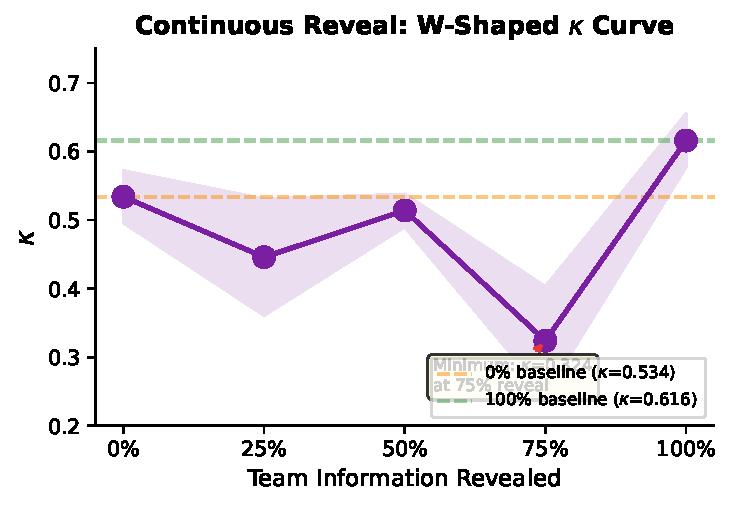
\includegraphics[width=\columnwidth]{figures/fig_reveal.pdf}
\caption{Continuous reveal $\kappa$ curve on 510K (PPO, 2 seeds/point, $10^6$ steps). $\kappa$ forms a W-shape: 75\% reveal is the global minimum ($\kappa=0.324$, 39\% below baseline).}
\label{fig:reveal}
\end{figure}

This finding has practical significance: \textit{incrementally improving an agent's information access can worsen training before improving it}.
$\kappa$ detects this regime, providing a diagnostic against premature or noisy information disclosure.


\section{Discussion}

\begin{table}[t]
\centering
\small
\setlength{\tabcolsep}{4pt}
\resizebox{\columnwidth}{!}{%
\begin{tabular}{lcccc}
\toprule
Condition & $\kappa$ & $\mathcal{P}$ & Regime & Result \\
\midrule
Toy REV.\  & 0.84 & Short  & Stable convergence   & Optimal \\
Toy HID.\  & 0.20 & Long   & Aimless drift        & Failure \\
OC STATIC  & 0.50 & ---    & Stable convergence   & Optimal \\
OC DYNAMIC & 0.00 & Short  & Info.\ stagnation    & Failure \\
510K A2C S & 0.64 & Medium & Product.\ exploration & Converged \\
510K A2C D & 0.52 & Short  & Conserv.\ convergence & Partial \\
\bottomrule
\end{tabular}}
\caption{Stable-or-Stuck classification across environments.
Short paths occur under both convergence (high $\kappa$) and stagnation (low $\kappa$).
Only the joint diagnostic discriminates.}
\label{tab:diagnosis}
\end{table}

\textbf{When does a short trajectory lie?}
Table~\ref{tab:diagnosis} synthesizes the three-environment evidence.
A short trajectory is honest when $\kappa$ is high (Toy \textsc{Revealed}, Overcooked \textsc{Static}).
It lies when $\kappa$ is low (Overcooked \textsc{Dynamic}: $\kappa=0$ across all eight seeds).
The intermediate case---510K \textsc{Dynamic}---retains partial gradient energy, but the short path overstates competence.

\textbf{$\kappa$ as a general-purpose diagnostic.}
$\kappa$ is lightweight, post-hoc, and algorithm-agnostic.
It provides three complementary signals: (1)~\textbf{direction}: $\kappa_R > \kappa_H$ indicates IIGC; (2)~\textbf{magnitude}: $\kappa \to 0$ signals complete gradient cancellation; (3)~\textbf{stability}: high $\kappa$ variance ($\sigma > 0.2$) predicts convergence failure.
Together with $\mathcal{P}$, $\kappa$ forms a diagnostic suite computable from any trained checkpoint without modifying the training pipeline.

\subsection{Case Study: Diagnosing a Noisy Sensor}

To demonstrate $\kappa$ as a practical engineering tool, we walk through a diagnosis-and-repair scenario using the continuous reveal data.

\textbf{Scenario.}
A practitioner is training PPO on 510K with hidden teammate information (0\% reveal baseline, $\kappa = 0.534$).
She adds a sensor that partially reveals teammate identity.
Due to noise, the sensor is only 75\% accurate.

\textbf{Symptom.}
After installing the sensor, training becomes \textit{worse}.
She computes $\kappa$:
\[
\kappa_{\text{before}} = 0.534 \quad \longrightarrow \quad \kappa_{\text{after}} = 0.324 \;\;(\text{39\% drop})
\]
The drop signals the sensor is \textit{increasing} gradient contraction.
The agent depends on the sensor's output, but the 25\% error rate causes destructive gradient updates when wrong---worse than having no sensor at all.

\textbf{Intervention.}
$\kappa$ suggests two fixes: (1)~Remove the sensor (return to $\kappa = 0.534$). (2)~Upgrade to fully reliable information ($\kappa = 0.616$, a 90\% improvement).

\textbf{Outcome.}
The practitioner implements Option 2.
After the fix, $\kappa$ rises from $0.324$ to $0.616$, and training stabilizes.
$\kappa$ served three roles: (1)~detecting harm, (2)~identifying the mechanism, (3)~verifying the intervention.

\textbf{Takeaway.}
This workflow---measure $\kappa$, diagnose, intervene, remeasure---positions $\kappa$ as a debugging tool for MARL system design.

\textbf{Limitations.}
$\kappa$ requires two identifiable hidden configurations; continuous hidden variables require discretization.
The path integral depends on feature design.
Cross-algorithm measurements are preliminary (SAC: 2 seeds).
Validation is restricted to three environments.

\textbf{Future work.}
Apply to standard MARL benchmarks (Hanabi, hidden-role games); develop online $\kappa$ monitoring; characterize $\kappa$ signatures for additional algorithm families (deterministic PG, QMIX); extend Pythagorean decomposition to $n$-way configurations.


\section{Conclusion}

We introduced Information-Induced Gradient Contraction (IIGC), a framework for understanding how hidden relational information erases learning signals in multi-agent RL.
The framework's centerpiece is $\kappa$, the Relational Gradient Retention Ratio---a single scalar measuring the fraction of gradient energy surviving partial observability.
Together with the path integral, $\kappa$ provides a Stable-or-Stuck diagnostic that classifies training trajectories into four regimes.

Three environments validate the framework: 510K reveals the deceptive pattern (hidden relations $\rightarrow$ shorter paths); Toy exposes diagnostic necessity (hidden relations $\rightarrow$ wandering with zero learning); Overcooked demonstrates power in a realistic setting ($\kappa=0.000$ across eight seeds).
Cross-algorithm measurements reveal systematic $\kappa$ signatures distinguishing policy-gradient from value-based methods.
A short trajectory can lie; $\kappa$ tells you when to believe it.


\end{document}
